\problem{Image Sharping}
(a) Let $\mathbf{a}=\begin{bmatrix}-1 & 0 & 1\end{bmatrix}^T$, and $\mathbf{b}=\begin{bmatrix}1 & 2 & 1\end{bmatrix}^T$.

Sobel operator among $x$ direction:
$S_x=\begin{bmatrix}
    -1 & -2 & -1 \\
    0 & 0 & 0 \\
    1 & 2 & 1
\end{bmatrix}=\begin{bmatrix}-1 \\ 0 \\ 1\end{bmatrix}\begin{bmatrix}1 & 2 & 1\end{bmatrix}= \mathbf{a}\mathbf{b}^T$

Sobel operator among $y$ direction:
$S_y=\begin{bmatrix}
    -1 & 0 & 1 \\
    -2 & 0 & 2 \\
    -1 & 0 & 1
\end{bmatrix}=\begin{bmatrix}1 \\ 2 \\ 1\end{bmatrix}\begin{bmatrix}-1 & 0 & 1\end{bmatrix}= \mathbf{b}\mathbf{a}^T$\\
So both the Sobel operators can be represented as the outer product of two vectors, i.e. its separable.\\
From what we have learned, if a separable filter can be represented as $\mathbf{w}= \mathbf{w}_1\mathbf{w}_2^T$, then the convolution of the filter with an image can be computed as $\mathbf{I}*\mathbf{w}=(\mathbf{I}*\mathbf{w}_1)*\mathbf{w}_2^T$, where `$*$' represents convolution.\\
So we can implement the separated kernels sequencially to the origin image to get the results.\\
The $S\_x\_a$ represents the convolution of origin image and $\mathbf{a}$, $S\_x\_ab$ represents convolution of $S\_x\_a$ and $\mathbf{b}^T$, which also means that the convolution of origin image and the $S_x$ operator.\\
And $S\_y\_b$ represents the convolution of origin image and $\mathbf{b}$, $S\_y\_ba$ represents convolution of $S\_y\_b$ and $\mathbf{a}^T$, which also means that the convolution of origin image and the $S_y$ operator.\\
Specifically, for the convenience of checking, the negative values are turned to $0$, and then the image pixel values are normalized to $[0, 255]$ after filtering.\\
And the results are shown in Figure \ref{fig:p1a}.\\

\begin{figure}[htbp]
    \centering
	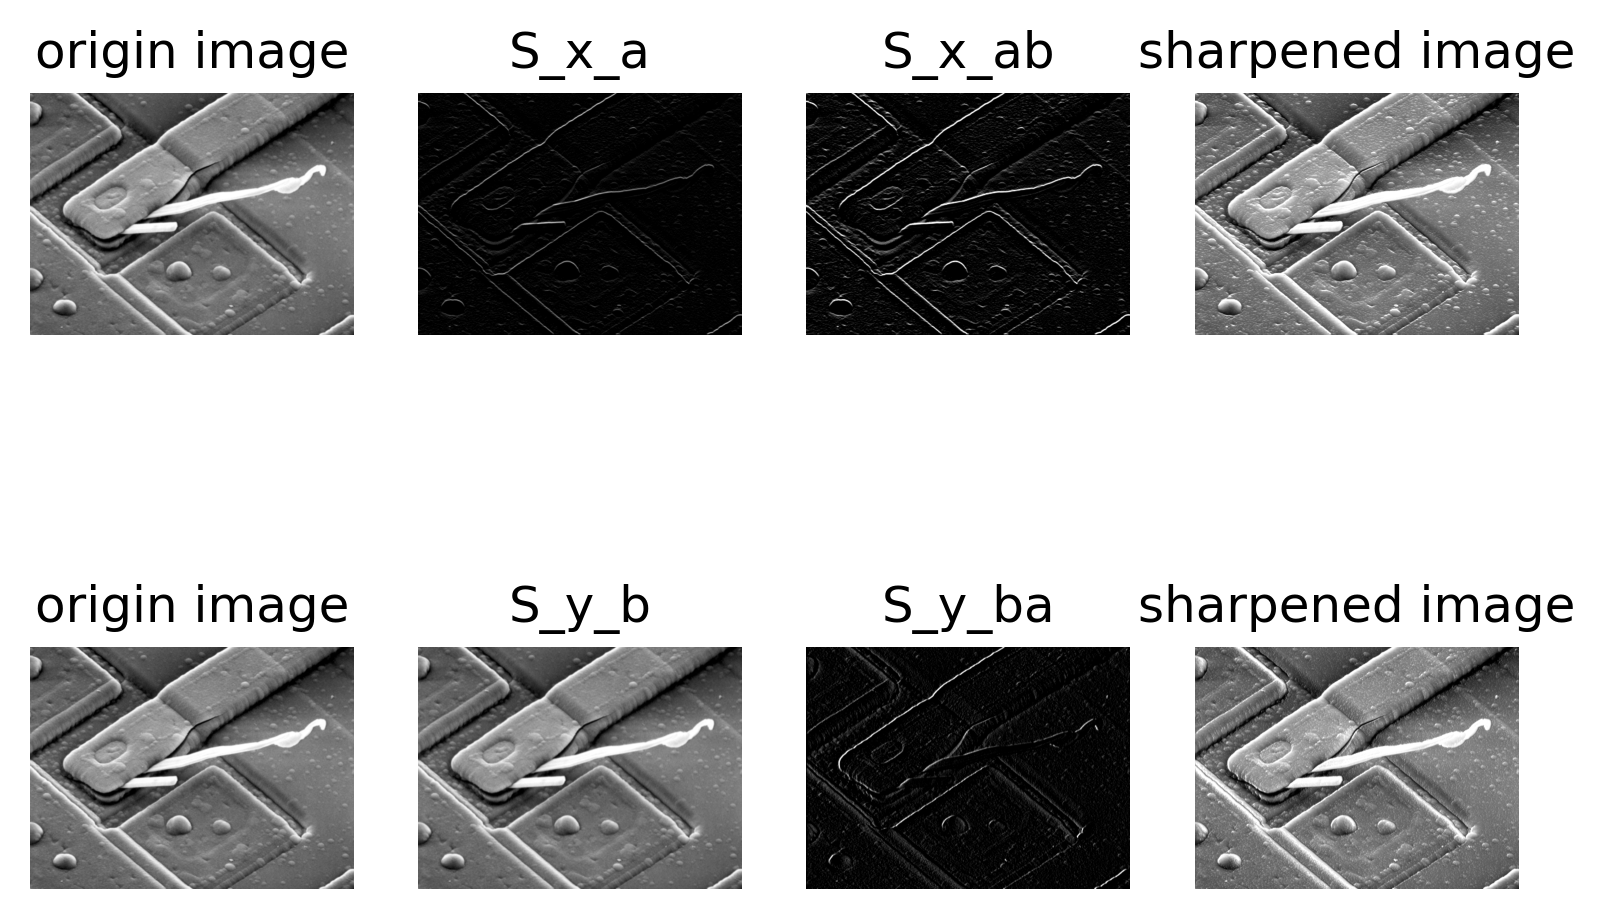
\includegraphics[width=\textwidth]{../images/p1/p1a.png}
    \caption{Processed images by Sobel operators among $x$ and $y$ directions.}
    \label{fig:p1a}
\end{figure}
We also tried to use the gradient of Sobel kernels to sharpen the image.\\
i.e.
$$G = \sqrt{(S\_x\_ab)^2 + (S\_y\_ba)^2}$$
The gradient of Sobel kernels and its sharpened image are shown in Figure \ref{fig:p1a_gradient}.\\
\begin{figure}[htbp]
    \centering
	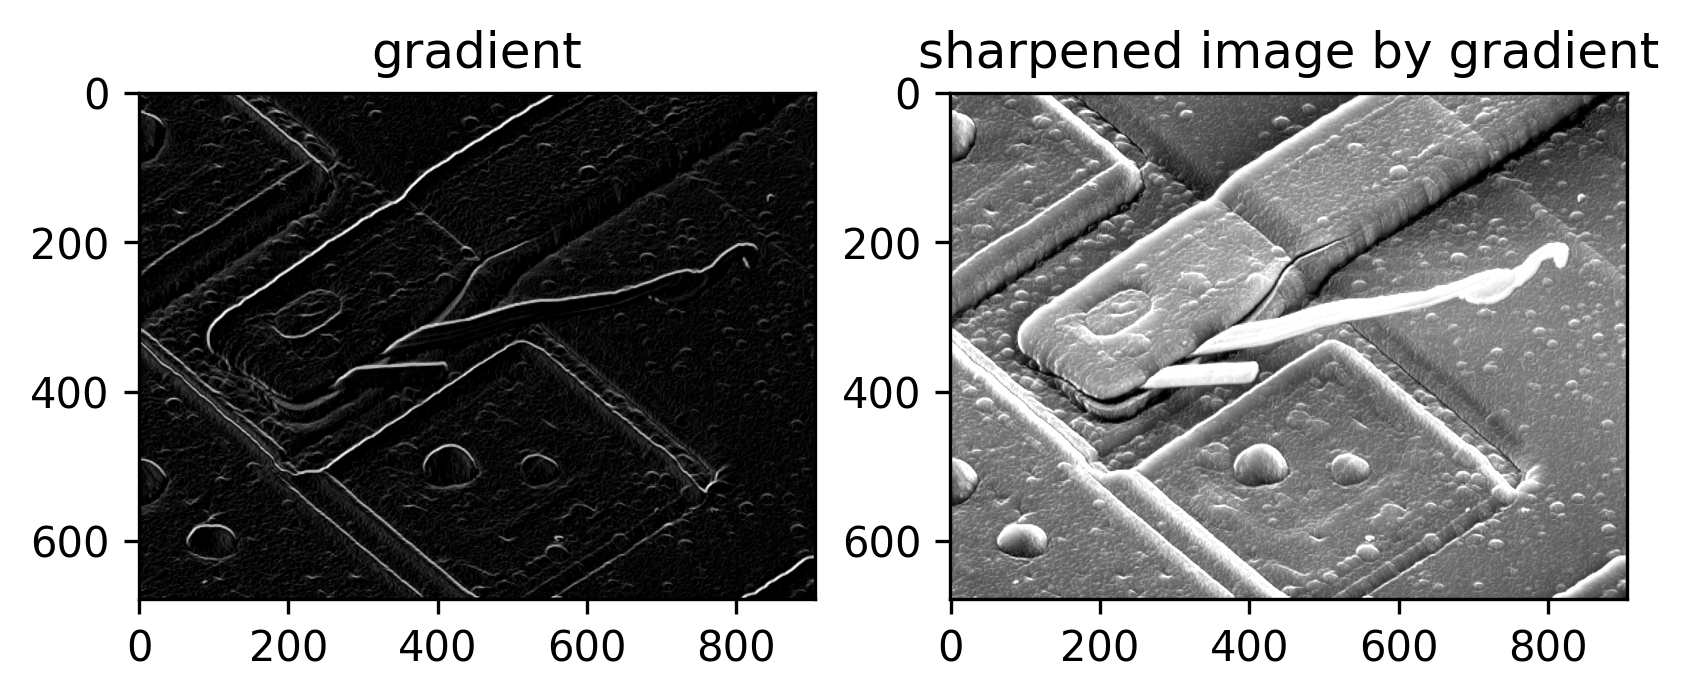
\includegraphics[width=\textwidth]{../images/p1/p1a_gradient.png}
    \caption{Sharpened by the gradient of Sobel kernels.}
    \label{fig:p1a_gradient}
\end{figure}


(b) Gaussian Highpass Filter:\\
The Gaussian Highpass Filter is:
$$H(u,v)=1-\exp\left(-\dfrac{D(u,v)^2}{2D_0^2}\right)$$
Where
$$D(u,v)=\left[\left(u-\dfrac{P}{2}\right)^2+\left(v-\dfrac{Q}{2}\right)^2\right]^\frac{1}{2}$$
In order to do FFT, we need to pad the image to the size of $2^m*2^n$, where $m$ and $n$ are integers.\\
So the images size varies: $678*906\Rightarrow 1024*1024$.
And aftering filtering, the image is cropped to the original size.

The Gaussian high pass filter is shown in Figure \ref{fig:p1b_Gaussian}.\\

\begin{figure}[htbp]
    \centering
	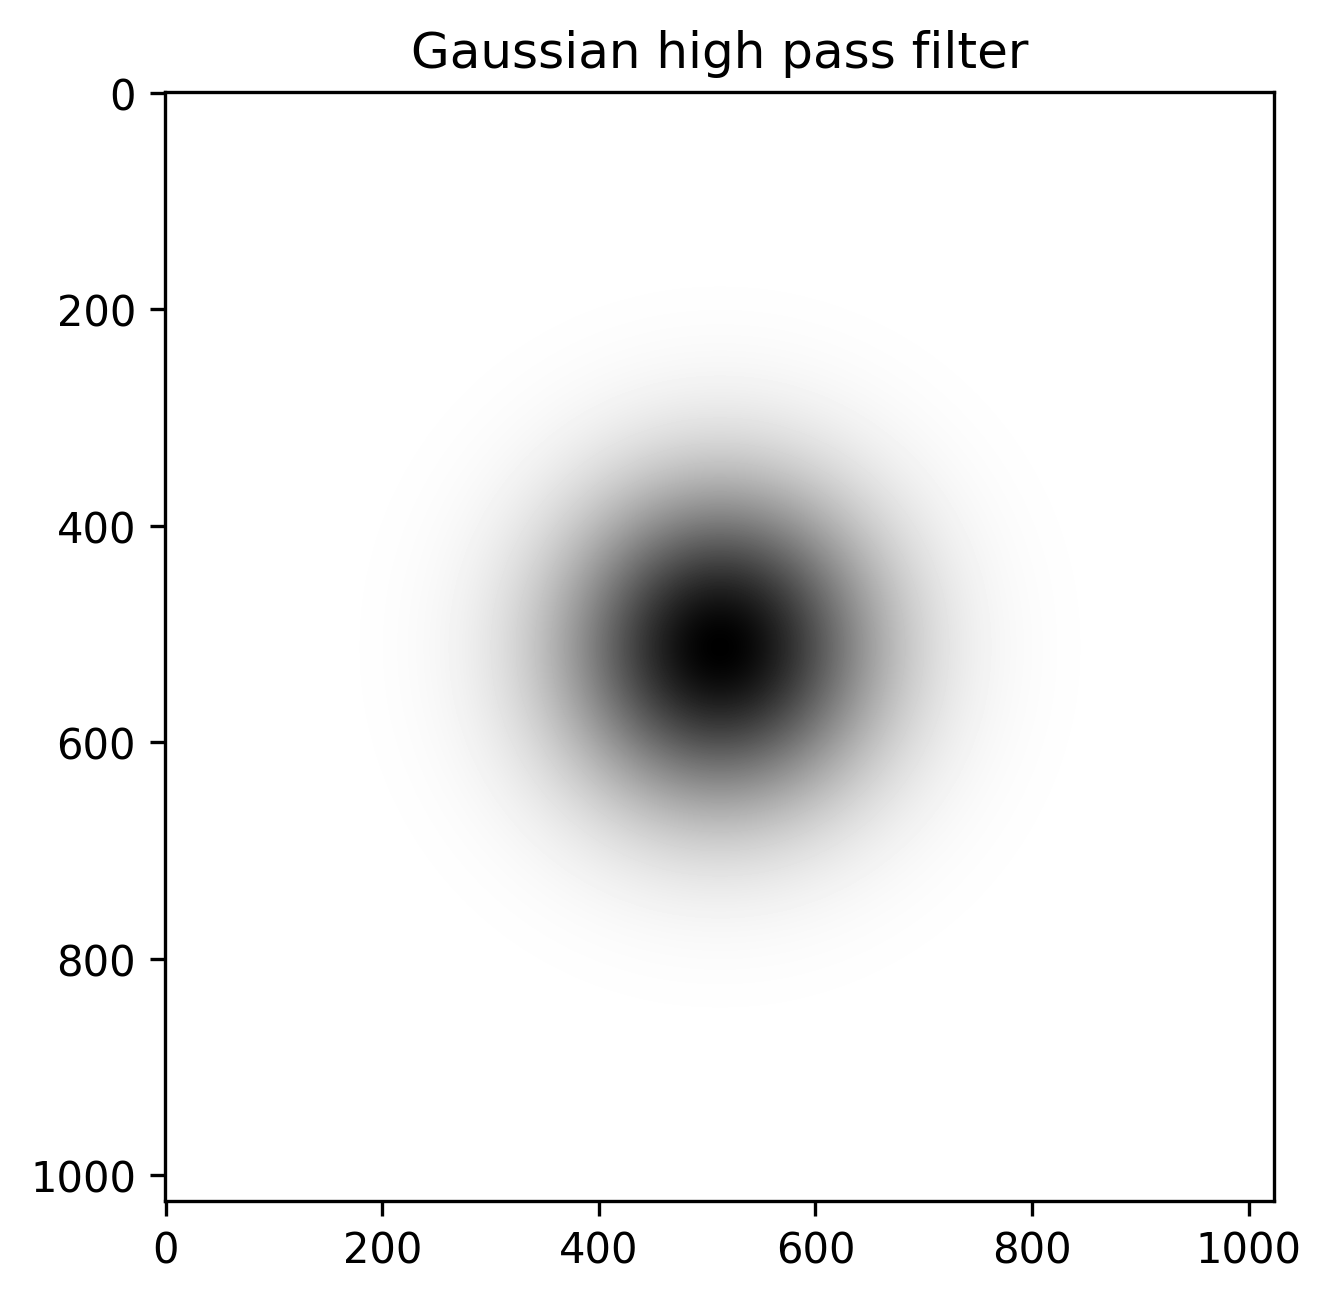
\includegraphics[width=0.4\textwidth]{../images/p1/p1b_Gaussian.png}
	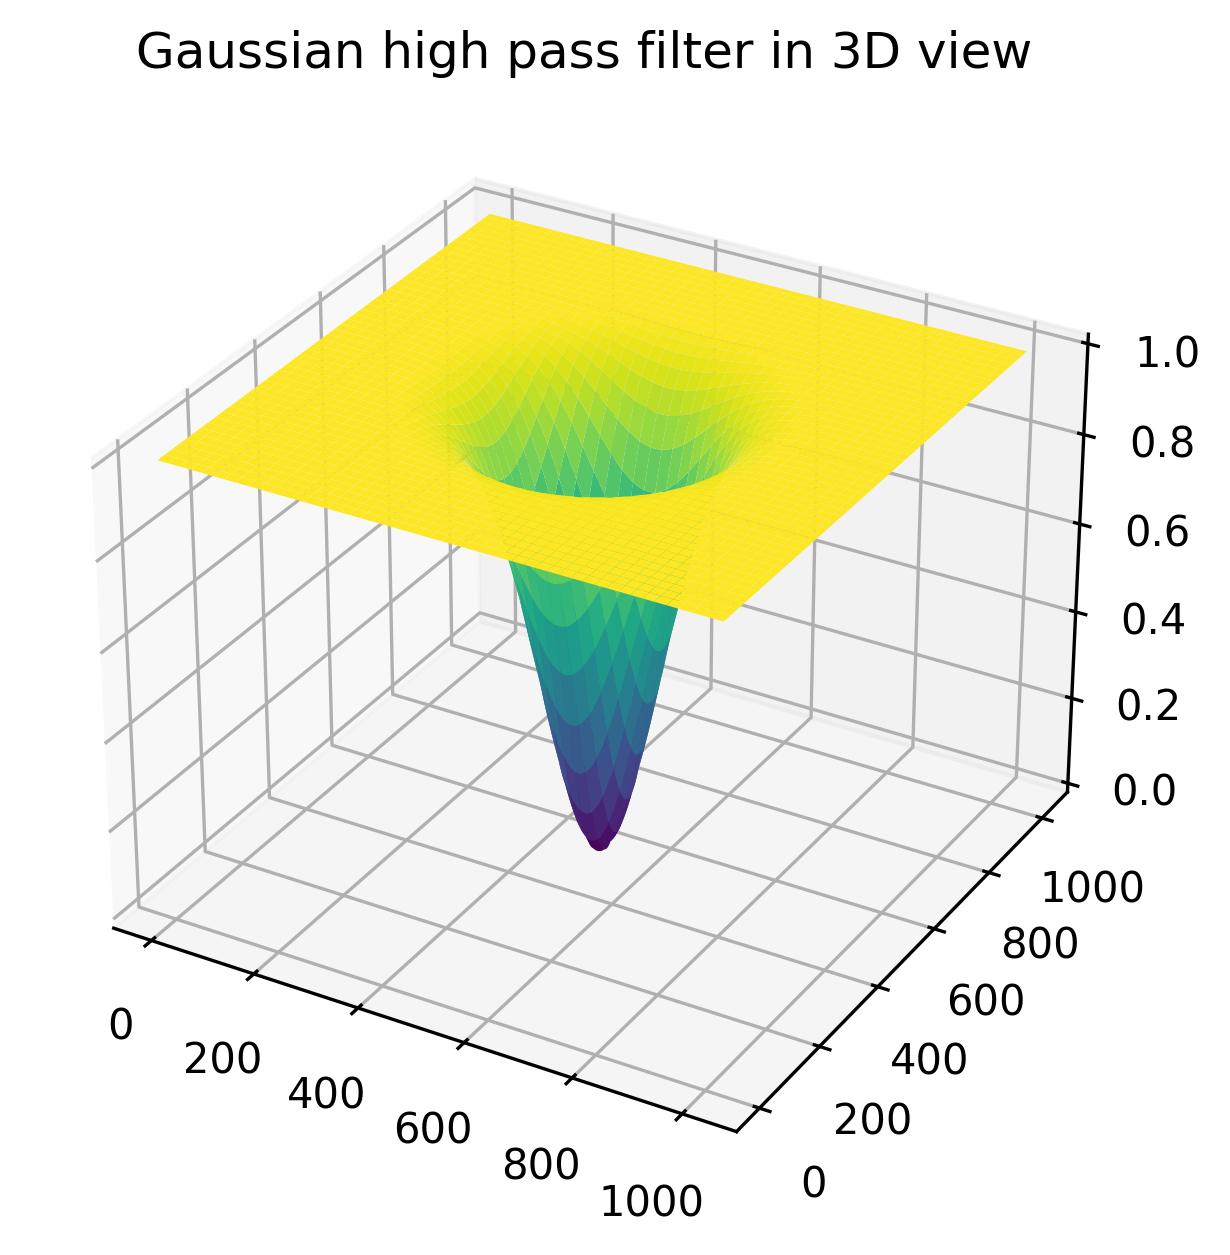
\includegraphics[width=0.4\textwidth]{../images/p1/p1b_Gaussian_3D.png}
    \caption{Gaussian high pass filter}
    \label{fig:p1b_Gaussian}
\end{figure}


To have a better effect of visualization on the frequency domain, the image is shown by applying the log transformation on the magnitude of the Fourier transform of the image.\\
i.e. $I_{\text{log}}=20\log(1+|I|)$, where $I$ is the spectrum generated by Fourier transform of the image.\\
The spectrum of the origin image and its filtered spectrum by the Gaussian highpass filter is shown in Figure \ref{fig:p1b_spectrum}.\\
The results of filtering the image with the Gaussian high pass filter and its sharpened image is shown in Figure \ref{fig:p1b_result}.\\
The filtered image is generated by using the inverse Fourier transform to the frequency domain results in the real domain.\\

\begin{figure}[htbp]
    \centering
	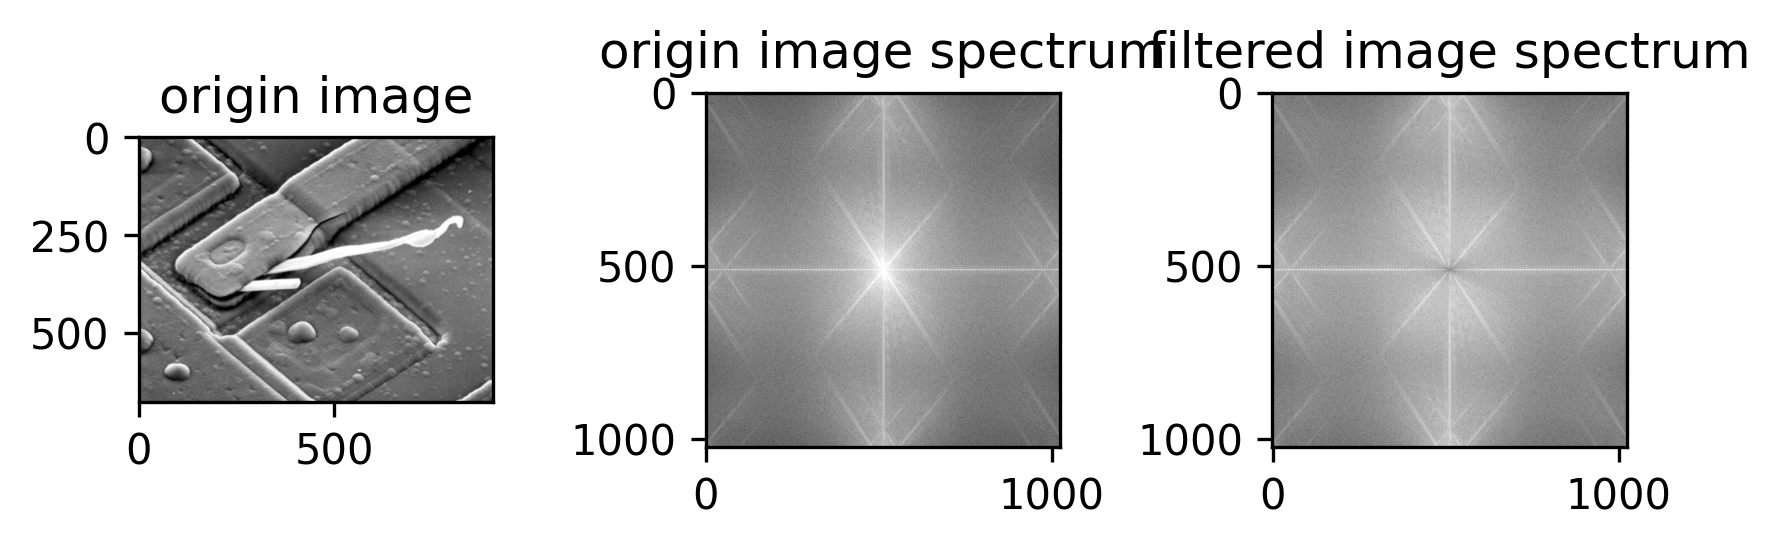
\includegraphics[width=\textwidth]{../images/p1/p1b_spectrum.png}
    \caption{Spectrum of Gaussian Highpass Filtered iamge.}
    \label{fig:p1b_spectrum}
\end{figure}

\begin{figure}[htbp]
    \centering
	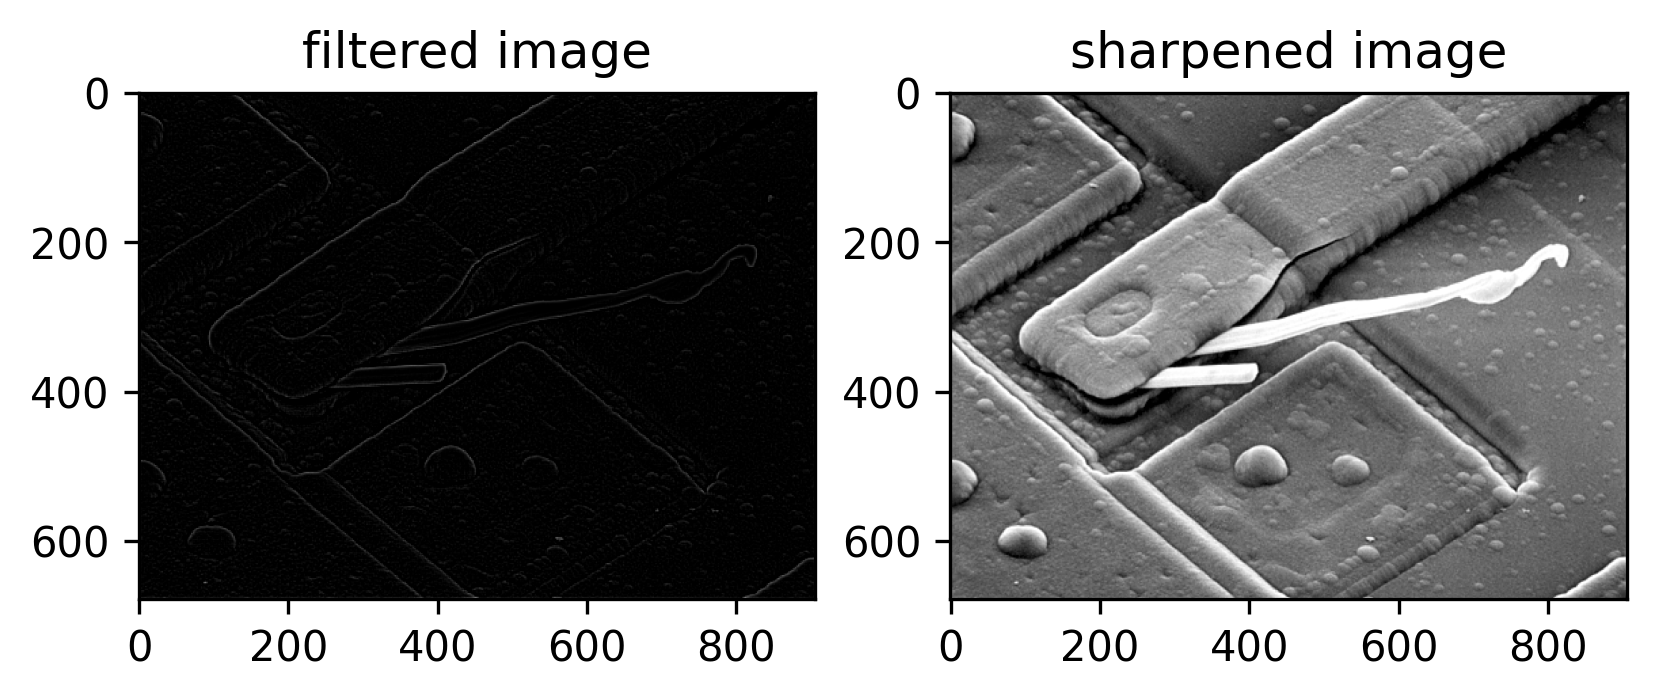
\includegraphics[width=0.9\textwidth]{../images/p1/p1b_result.png}
    \caption{Results of filtering the image with the Gaussian high pass filter.}
    \label{fig:p1b_result}
\end{figure}

\newpage